\documentclass[11pt]{article}
\usepackage[margin=1in]{geometry}
\usepackage[T1]{fontenc}
\usepackage{lmodern}
\usepackage{amsmath}
\usepackage{booktabs}
\usepackage{graphicx}
\usepackage{xurl}
\usepackage[hidelinks]{hyperref}
\emergencystretch=2em

\title{The August excess of US-born major leaguers is not seen in the cohorts born after the 2006 youth-baseball cutoff change: a pre-registered test}
\author{Qianghao Wu}
\date{28 November 2026}

\begin{document}
\maketitle

\begin{abstract}
\noindent G.~Spira (Slate, 2008) counted 503 August and 313 July births among US-born major leaguers and attributed the excess to the July~31 age cutoff of US youth baseball. Little League moved the cutoff to April~30 from the 2006 season. We pre-registered a test of whether the ratio of August--October to May--July births changed between US-born players born from August 1976 to July 1992 (July~31 rule at league ages 9 to 12) and those born from May 1996 to April 2001 (April~30 rule at those ages). The data are the MLB Stats API player lists for the seasons 1985--2026. A player counts only if he debuted before age 25, so that every birth month has the same time to reach the major leagues. The ratio is $445/304 = 1.46$ in the earlier cohort and $112/112 = 1.00$ (95\% interval 0.77 to 1.30) in the later cohort. The odds ratio is 1.46 (95\% CI 1.08 to 1.98), one-sided Fisher $p = 0.0079$. A placebo split of the earlier cohort gives $p = 0.74$. By the pre-registered rule, the result supports a change. Spira's predicted May peak is not seen. Exploratory analyses limit the result. The fall starts about three birth years before the later cohort, with players who played most or all of league ages 9 to 12 under the old rule, so the data cannot place the effect at those ages. With a debut limit of 24 instead of 25, the change is not significant ($p = 0.29$). Players born outside the USA show no excess and no change, and US birth seasonality predicts an odds ratio of 1.002. The result is an association across birth cohorts. This work has not yet been reviewed by experts. The computations, the code and the text were produced by AI models (from Anthropic and OpenAI), working under the author's direction.
\end{abstract}

\section{Introduction}

A relative age effect occurs when an age group uses a single cutoff date: children born just after the cutoff are the oldest of their group, and selection for skill favours them. An early paper on the effect in Major League Baseball (MLB) is ``Born to Play Ball'' by Thompson, Barnsley and Stebelsky~\cite{thompson1991} (we read only its bibliographic record). For US youth baseball, the cutoff was July~31 for more than 55 years~\cite{ll2005}. So August births are the oldest and July births are the youngest of an age group.

Spira~\cite{spira2008} gave the best-known count. As of the 2005 season, 503 US-born major leaguers born in August and 313 born in July had reached the major leagues (players born since 1950). He reported that USA Baseball moved the date from July~31 to April~30, and he wrote: ``Future Juan Pierres, take note: If you want to make it in the majors, forget about August. Make sure you're born in May.'' Little League announced in October 2005 that ``starting with the 2006 season, the date in all divisions of Little League Baseball will be April~30''~\cite{ll2005}. An article on Bill James Online~\cite{jedlovec2009} reports that Dixie Youth also moved from July~31 to April~30 for 2006, that some organizations did not move, and that most school teams group players by grade. That author also expected the advantage to move to May. Little League moved the date again, to August~31, from the 2018 season~\cite{ll2015}.

The 2006 change is a natural experiment. The youth-league cutoff moved by three months. School teams group players by grade~\cite{jedlovec2009}, and that grouping did not change in 2006. US birth seasonality differs little between the two cohorts (Section~\ref{sec:explore}). An article on the Omni Calculator site~\cite{siuda} repeats Spira's counts and says that ``only a fresh count will show whether the August advantage has faded.'' The year of that article is not stated on the page.

\paragraph{Prior work.}
Abel and Kruger~\cite{abel2005} studied MLB players active 1880--1999. By their abstract, Aug--Oct births were over-represented from 1900 on, the distribution matched that of the general population before 1980, and the excess became larger after 1980; they attribute the later excess to Little League and its August~1 date. Zhang, Lemez, Wattie and Baker~\cite{zhang2018} studied 16{,}122 American-born players of the seasons 1871--2014 and found a significant effect for players born 1950--1970 (abstract). Herring, Beyer and Fukuda~\cite{herring2021} studied 7{,}078 players of the 2013--2018 MLB drafts. By their abstract, the quarter Aug--Oct was over-represented ($z = +4.45$) and the quarter Feb--Apr was under-represented ($z = -4.15$); the abstract reports no split by birth year and no before/after contrast. We could not read their full text (paywall). A Clemson master's thesis~\cite{hensley2020} compares birth months in the NHL, NBA and MLB with the general population (abstract). A blog post~\cite{collier2016} confirms a non-uniform birth-month distribution of MLB players with a $\chi^2$ test. Duda~\cite{duda2026} locates the cutoff of US-born MLB players born from 1951 at July~29 from their birth dates, against Little League's July~31; we found no split of the MLB players by birth year and no test of the 2006 change in it. Spira~\cite{spira2008} and Jedlovec~\cite{jedlovec2009} used data to 2005 and 2009, before any player of the new rule could debut.

\paragraph{Contribution.}
We found no published before/after test, by birth cohort, of the birth months of US-born major leaguers across the 2006 change. This paper gives such a test. It was pre-registered, it has placebo and shuffle controls, and its data are public. A search cannot prove absence; Section~\ref{sec:limits} lists the searches.

\section{Data}

The MLB Stats API~\cite{statsapi} gives, for each season, the list of players with \texttt{id}, \texttt{birthDate}, \texttt{birthCountry} and \texttt{mlbDebutDate}. We downloaded the seasons 1985--2026 on 28 November 2026 and took the union by \texttt{id}. We keep players with \texttt{birthCountry} equal to \texttt{USA} and with a birth date and a debut date. Of 9876 players, 98 have no debut date.

\paragraph{Cohorts.} Each cohort covers whole years of 12 months, so the window does not favour any month.
\begin{itemize}
\item Control C: born 1976-08-01 to 1992-07-31. The July~31 rule applied at all league ages 9 to 12.
\item Treatment T: born 1996-05-01 to 2001-04-30. The April~30 rule applied at all league ages 9 to 12.
\end{itemize}
The players born 1992-08 to 1996-04 are outside both cohorts. We call those born 1992-08-01 to 1995-07-31 the gap cohort.

\paragraph{Equal exposure.} A player counts only if his debut is before his 25th birthday. The 25th birthday of every T player is on or before 2026-04-30, so the full window is observed for every T player. Without this rule, players born early in the last birth year of T would have had more time to debut.

\section{Pre-registered test}

The protocol (file \texttt{PROTOCOL.md}) was committed before the outcome files. Only the commit order proves this: the protocol commit \texttt{0569aaa} (02:23:35) is 3 minutes before the commit of the analysis script and the expected numbers (\texttt{bfc9b7a}, 02:26:30). The raw season files were on disk before the protocol commit. That no birth-month count was made before the protocol commit is the statement of the session that wrote it; no log proves it. Two dated addenda record later changes; no rule of the test changed.

\paragraph{Primary test.} Let group A be the birth months May, June and July, and group B be August, September and October. Under the July~31 rule, B holds the oldest and A the youngest children of an age group. Under the April~30 rule, May--July are the oldest. The test uses the $2\times2$ table cohort (T, C) $\times$ group (A, B), with odds ratio
\[
\mathrm{OR} = \frac{A_T / B_T}{A_C / B_C}.
\]
The test is a one-sided Fisher exact test of $\mathrm{OR} > 1$ at the threshold $p < 0.05$. The 95\% confidence interval of $\log \mathrm{OR}$ uses the Woolf (normal) method.

\paragraph{Controls.}
(1) Placebo split: C1 born 1976-08 to 1984-07 against C2 born 1984-08 to 1992-07, with no change of cutoff; we expect $p \ge 0.05$.
(2) Other months: Nov--Jan against Feb--Apr, T against C.
(3) A shuffle of the cohort labels, 20{,}000 permutations, seed 20261128.
(4) A known answer: in C, August births must outnumber July births.

\paragraph{Decision rule.} SUPPORT if the primary $p < 0.05$ and the placebo split $p \ge 0.05$. REFUTE if the upper end of the 95\% CI of $\log\mathrm{OR}$ is below $\log r_C$, where $r_C = B_C/A_C$; this excludes a transfer of half the excess. Otherwise INCONCLUSIVE.

\section{Results}

\begin{table}[ht]
\centering
\caption{Primary table. US-born players with an MLB debut before age 25.}
\label{tab:primary}
\begin{tabular}{llrrrr}
\toprule
Cohort & Born & $n$ & May--Jul (A) & Aug--Oct (B) & B/A \\
\midrule
C (July 31 rule) & 1976-08-01 to 1992-07-31 & 1341 & 304 & 445 & 1.46 \\
T (April 30 rule) & 1996-05-01 to 2001-04-30 & 394 & 112 & 112 & 1.00 \\
\bottomrule
\end{tabular}
\end{table}

Table~\ref{tab:primary} gives the counts. The monthly counts, January to December, are 98, 94, 96, 100, 111, 101, 92, 148, 174, 123, 96, 108 for C and 22, 32, 16, 25, 40, 32, 40, 41, 41, 30, 45, 30 for T (Figure~\ref{fig:main}, right).

\begin{itemize}
\item Primary: $\log\mathrm{OR} = 0.381$, OR 1.46, 95\% CI 1.08 to 1.98 ($\log$: 0.081 to 0.681). One-sided Fisher $p = 0.0079$.
\item Shuffle of cohort labels: one-sided $p = 0.0085$, in agreement with the Fisher test.
\item Placebo split of C: 152/232 (C2) against 152/213 (C1), $\log\mathrm{OR} = -0.085$ (CI $-0.377$ to $0.206$), $p = 0.74$.
\item Known answer in C: 148 August against 92 July births, two-sided binomial $p = 0.00036$. Spira's pattern is present in C.
\item Control 2, Nov--Jan against Feb--Apr: 97/73 in T against 302/290 in C, $\log\mathrm{OR} = 0.244$ (CI $-0.100$ to $0.588$), two-sided $p = 0.19$. This control is not neutral. The protocol said that the cutoff change predicts nothing for these months. That was wrong: under an April~30 cutoff, Feb--Apr births are the youngest, so the change predicts a fall of Feb--Apr against Nov--Jan. The observed direction agrees with that, but it is not significant. We do not use this control as evidence about a general change of month shares.
\item Decision: SUPPORT.
\end{itemize}

In T, the ratio B/A is $112/112 = 1.00$ with an approximate 95\% interval of 0.77 to 1.30. So the data do not exclude a remaining Aug--Oct excess of up to about 1.3. The point estimate $\log\mathrm{OR} = 0.381$ equals $\log r_C$, the ``half transfer'' value of the protocol. This equality is an identity when $A_T = B_T$; it is not separate evidence. Spira's stronger prediction, a May peak, is not seen: T has 40 May and 41 August births.

\begin{figure}[ht]
\centering
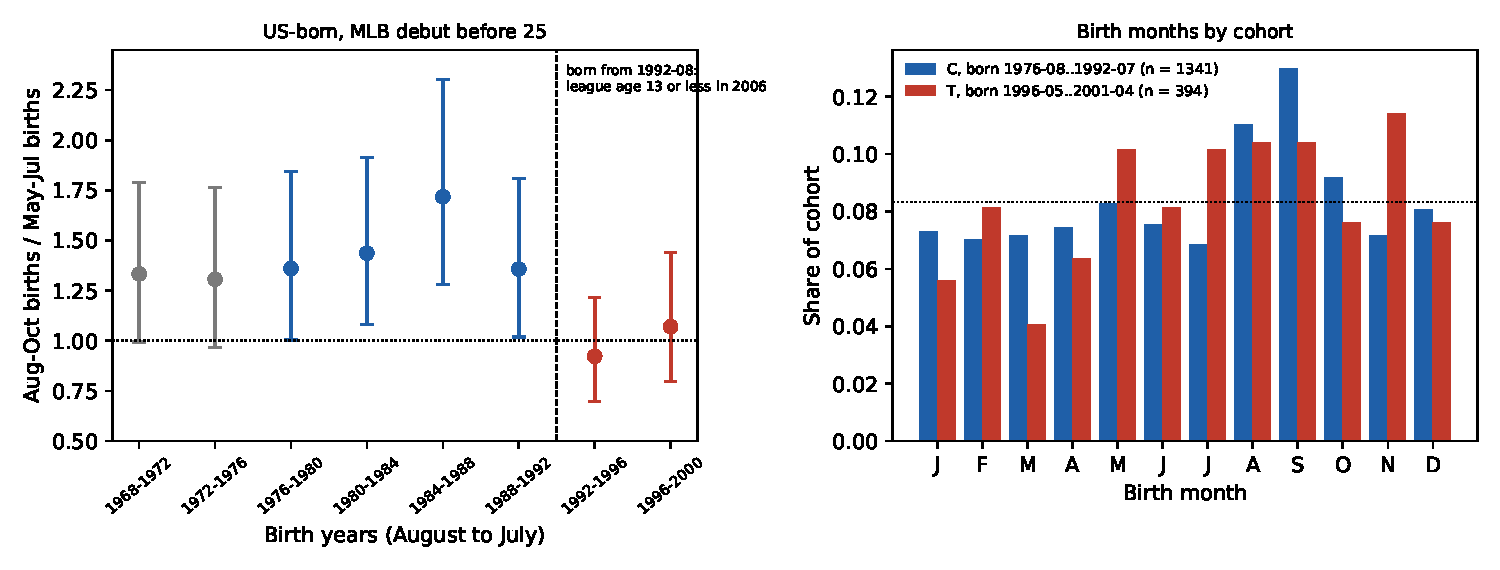
\includegraphics[width=\textwidth]{figures/fig1.pdf}
\caption{Left: ratio of Aug--Oct to May--Jul births by four-year birth bin (August to July), US-born players with a debut before age 25, with 95\% intervals. Blue: cohort C. Red: born from August 1992 to July 2000 (the gap cohort and most of T). Grey: earlier births, outside the test. Right: share of each birth month in cohorts C and T. The dotted line is 1/12.}
\label{fig:main}
\end{figure}

\section{Exploratory analyses}\label{sec:explore}

The analyses in this section were added after the primary result. They are not pre-registered. Most were requested by an independent check of the first result.

\begin{table}[ht]
\centering
\caption{Aug--Oct / May--Jul by birth bin (August to July). US-born, debut before 25.}
\label{tab:bins}
\begin{tabular}{lrrr}
\toprule
Born & May--Jul & Aug--Oct & ratio \\
\midrule
1968-08 to 1972-07 & 78 & 104 & 1.33 \\
1972-08 to 1976-07 & 75 & 98 & 1.31 \\
1976-08 to 1980-07 & 72 & 98 & 1.36 \\
1980-08 to 1984-07 & 80 & 115 & 1.44 \\
1984-08 to 1988-07 & 71 & 122 & 1.72 \\
1988-08 to 1992-07 & 81 & 110 & 1.36 \\
1992-08 to 1996-07 & 104 & 96 & 0.92 \\
1996-08 to 2000-07 & 85 & 91 & 1.07 \\
\bottomrule
\end{tabular}
\end{table}

\paragraph{Timing.} Table~\ref{tab:bins} and Figure~\ref{fig:main} (left) show that the ratio falls with the players born from August 1992, about three birth years before T. Single birth years (May--Jul/Aug--Oct) are 16/25 for 1991--92, 20/25 for 1992--93, 35/25 for 1993--94, 22/27 for 1994--95, 27/19 for 1995--96, 19/25 for 1996--97, 22/23 for 1997--98, 22/26 for 1998--99 and 22/17 for 1999--2000. These counts are small and noisy, so the data cannot fix the first birth year of the change. The gap cohort (born 1992-08 to 1995-07) has 77 May--Jul and 77 Aug--Oct births. Against C its OR is 1.46 (95\% CI 1.03 to 2.07), one-sided $p = 0.020$. T does not differ from the gap cohort (OR 1.00, CI 0.66 to 1.51, $p = 0.54$).

The players born 1992-08 to 1994-07 were league age 11 to 13 in 2006 (age on April~30). They played most or all of league ages 9 to 12 under the July~31 rule. Those born 1992-08 to 1993-04 had no season at league ages 9 to 12 under the new rule. So the data cannot place the effect at league ages 9 to 12, as the protocol assumed. One possibility is that the April~30 rule also acts at older youth ages, for example in 13-and-over divisions and in travel baseball. We did not test this. Two facts weaken it. First, US high-school and college baseball group players by school year~\cite{jedlovec2009}, and that did not change in 2006. Second, the single birth years are noisy, as above.

\paragraph{Pre-trend.} Inside C, a Cochran--Armitage trend test of the share of May--Jul over 16 single birth years gives $z = -0.19$, two-sided $p = 0.85$. So the fall after 1992 does not continue an earlier trend. T against the later half of C (born 1984-08 to 1992-07; 152/232) gives OR 1.53 (CI 1.10 to 2.13), $p = 0.0079$.

\paragraph{Debut-age limit.} Table~\ref{tab:age} varies the debut-age limit of the equal-exposure rule. For the limits 26 and 27, T ends at 2000-04-30 and 1999-04-30, so that the full window stays observed. The rows are nested samples of the same players; they are not independent tests. The change is significant for the limits 23, 25, 26 and 27. It is not significant for the limit 24 (OR 1.15, $p = 0.29$) or the limit 22 ($p = 0.23$, with only 15 T players in groups A and B). The pre-registered limit is 25.

\begin{table}[ht]
\centering
\caption{Sensitivity to the debut-age limit (exploratory). The rows are nested, not independent. A/B counts are May--Jul/Aug--Oct.}
\label{tab:age}
\begin{tabular}{lrrrrr}
\toprule
Debut before & T: A/B & C: A/B & OR & 95\% CI & one-sided $p$ \\
\midrule
22 & 7/8 & 32/65 & 1.78 & 0.59--5.34 & 0.23 \\
23 & 23/21 & 86/158 & 2.01 & 1.05--3.84 & 0.025 \\
24 & 49/64 & 185/278 & 1.15 & 0.76--1.74 & 0.29 \\
25 (primary) & 112/112 & 304/445 & 1.46 & 1.08--1.98 & 0.0079 \\
26 (T to 2000-04) & 132/132 & 424/596 & 1.41 & 1.07--1.84 & 0.0085 \\
27 (T to 1999-04) & 129/136 & 501/685 & 1.30 & 0.99--1.69 & 0.033 \\
\bottomrule
\end{tabular}
\end{table}

\paragraph{Players not born in the USA.} With the same cohorts and rules, players not born in the USA have 55/56 (T) against 143/155 (C), OR 1.07 (CI 0.69 to 1.65), two-sided $p = 0.82$. This group shows no Aug--Oct excess in C and no change. The data hold only the birth country. Our assumption is that most of these players did not play US youth baseball; some of them grew up in the USA. With this assumption, the control agrees with a US-specific cause.

\paragraph{Other month groups.} July against August only: 40/41 against 92/148, OR 1.57 (CI 0.95 to 2.61), $p = 0.053$. Jun--Jul against Aug--Sep: OR 1.47 (CI 1.02 to 2.11), $p = 0.025$. Apr--Jul against Aug--Nov: OR 1.17 (CI 0.90 to 1.52), $p = 0.14$.

\paragraph{Leave one year out.} When we remove one birth year of T at a time, the one-sided $p$ goes from 0.0066 to 0.029. No single birth year carries the result.

\paragraph{US birth seasonality.} If players were drawn in proportion to US male births by month (CDC and NCHS counts~\cite{cdcbirths}), the ratio of Aug--Oct to May--Jul births would be 1.017 in the C window and 1.015 in the T window. The expected OR is 1.002. So a change of birth seasonality explains almost none of the observed OR of 1.46.

\section{How the numbers were checked}

The script \texttt{checks/rerun.py} downloads the 42 season lists and the CDC file, computes every number in this paper, and compares the result with \texttt{data/expected.json}. It uses the Python standard library only. The Fisher tests use exact rational arithmetic. A run from a fresh download on 28 November 2026 printed ``MATCH expected.json''.

An independent check, in two rounds, did the following:
\begin{itemize}
\item It reran the script from a clean copy of the repository and a fresh download. The result was ``MATCH expected.json''.
\item It recounted the primary table with its own code (SciPy Fisher test): 112/112 against 304/445, OR 1.464, $p = 0.0079$.
\item It recounted the primary table from a second source, the Retrosheet biographical file~\cite{retrosheet}: 113/112 against 303/445, OR 1.48, $p = 0.0062$. The gap cohort is also 77/77 in that source.
\item It recounted every exploratory number with its own standard-library code: all values agree.
\item It compared the CDC seasonality with a second birth-count file (FiveThirtyEight, 1994--2003, both sexes): ratio 1.0179 against 1.0181.
\end{itemize}
The scripts of the independent check are in \texttt{checks/verify/}.

\section{Limits}
\label{sec:limits}

\begin{itemize}
\item The result is an association across birth cohorts. The design does not remove other changes of the same period, for example travel-ball organizations with other cutoffs, or changes in scouting and the draft.
\item The fall of the ratio starts about three birth years before T. The data cannot place the effect at league ages 9 to 12, and they cannot tell an effect at teen ages from other causes of that period.
\item T is small (394 players; 224 in groups A and B). The T ratio has a 95\% interval of 0.77 to 1.30, so a remaining excess of up to about 1.3 is not excluded.
\item The result depends on the debut-age limit (Table~\ref{tab:age}).
\item Herring et al.~\cite{herring2021} still find an Aug--Oct excess among 2013--2018 draftees taken as one group. Their group mixes birth cohorts and countries, and it includes players who never reach MLB, so it does not conflict with our result. We read only their abstract.
\item Cohorts born from 2001 were under April~30 and, from 2018, under August~31. An August~31 rule predicts a September peak. With the equal-exposure rule, these cohorts are not yet observable.
\item The MLB Stats API can correct its records. A later download can give different counts.
\item Novelty: searches of two collections of AI-produced results, of Zenodo, and of the web (terms: ``relative age effect'' with MLB, ``birth month'' with ``Little League'', the 2006 April~30 change) found no before/after test. A search cannot prove absence.
\end{itemize}

\section{Conclusion}

Among US-born players who reached MLB before age 25, the Aug--Oct excess of the cohort born 1976--1992 (ratio 1.46) is not seen in the cohort born 1996--2001 (ratio 1.00, 95\% interval 0.77 to 1.30). The change passes the pre-registered test (OR 1.46, $p = 0.0079$) and its placebo. The excess did not become a May peak. The change starts with players born from August 1992, earlier than the protocol assumed, and it is not significant with a debut limit of 24. The direction of the change agrees with a youth-cutoff effect. Its timing does not match the protocol's assumption, and the data do not prove that the cutoff caused the change.

\begin{thebibliography}{99}

\bibitem{spira2008} G.~Spira, ``The Boys of Late Summer,'' \emph{Slate}, 16 April 2008. \url{http://www.slate.com/articles/sports/sports_nut/2008/04/the_boys_of_late_summer.html}

\bibitem{thompson1991} A.~H.~Thompson, R.~H.~Barnsley and G.~Stebelsky, ``\,`Born to Play Ball': The Relative Age Effect and Major League Baseball,'' \emph{Sociology of Sport Journal} 8(2):146--151, 1991. doi:10.1123/ssj.8.2.146. (Bibliographic record only.)

\bibitem{abel2005} E.~L.~Abel and M.~L.~Kruger, ``Seasonality of birth in the majors, 1880--1999,'' \emph{Biodemography and Social Biology} 52(1--2):47--55, 2005. doi:10.1080/19485565.2002.9989098. (Abstract, PMID 17619630.)

\bibitem{zhang2018} B.~Zhang, S.~Lemez, N.~Wattie and J.~Baker, ``A historical examination of relative age effects in Major League Baseball,'' \emph{International Journal of Sport Psychology} 49(5):448--463, 2018. doi:10.7352/IJSP.2018.49.448. (Abstract.)

\bibitem{herring2021} C.~H.~Herring, K.~S.~Beyer and D.~H.~Fukuda, ``Relative Age Effects as Evidence of Selection Bias in Major League Baseball Draftees (2013--2018),'' \emph{Journal of Strength and Conditioning Research} 35(3):644--651, 2021. doi:10.1519/JSC.0000000000003951. (Abstract.)

\bibitem{hensley2020} C.~J.~Hensley, ``The Presence of the Relative Age Effect in Professional Sports,'' MA thesis, Clemson University, 2020. \url{https://open.clemson.edu/all_theses/3438}

\bibitem{jedlovec2009} B.~Jedlovec, ``The `Matthew Effect': The Impact of Birth Date on Baseball Success,'' Bill James Online, 4 November 2009. Archived copy: \url{http://web.archive.org/web/20230531162307/https://www.billjamesonline.com/article1191/}

\bibitem{collier2016} A.~Collier, ``Major League Baseball Birth Months,'' R-bloggers, 5 July 2016. \url{https://www.r-bloggers.com/2016/07/major-league-baseball-birth-months/}

\bibitem{duda2026} J.~Duda, ``HCR for statistical verification of folk regularities,'' Zenodo, 18 November 2026. doi:10.5281/zenodo.24348797.

\bibitem{siuda} D.~Siuda, ``503 major leaguers were born in August, only 313 in July,'' Omni Calculator (year not stated on the page). \url{https://www.omnicalculator.com/insights/sports/503-major-leaguers-were-born-in-august-only-313-in-july}

\bibitem{ll2005} Little League Baseball, questions and answers on the change of the league age determination date, October 2005. Archived copy: \url{http://web.archive.org/web/20051223154010/http://www.littleleague.org:80/media/age_change_Oct05.asp}

\bibitem{ll2015} Little League Baseball, ``Update to the Implementation of Little League Baseball Age Determination Date,'' 13 November 2015. \url{https://www.littleleague.org/news/update-implementation-little-league-baseball-age-determination-date/}

\bibitem{statsapi} MLB Stats API, season player lists, \url{https://statsapi.mlb.com/api/v1/sports/1/players?season=YYYY}, seasons 1985--2026, accessed 28 November 2026.

\bibitem{cdcbirths} J.~VanderPlas, US births by year, month and sex, 1969--2008, compiled from the CDC/NCHS natality files. \url{https://github.com/jakevdp/data-CDCbirths}

\bibitem{retrosheet} Retrosheet, biographical file (\texttt{biofile.zip}), file date 2026-08-07. \url{https://www.retrosheet.org/biofile.zip}. The information used here was obtained free of charge from and is copyrighted by Retrosheet.

\end{thebibliography}
\end{document}
